\documentclass[12pt]{article}

\usepackage{latexsym,amssymb,amsthm,amsmath,amscd,multirow,marvosym,fixltx2e,tikzsymbols}

\usepackage{tikz,latexsym,amssymb,amsthm,amsmath,amscd,multirow,marvosym,mathrsfs,fixltx2e}
\usetikzlibrary{svg.path}


\setlength{\oddsidemargin}{0cm}
\setlength{\evensidemargin}{0cm}
\setlength{\textwidth}{6.5in}
\setlength{\headheight}{-.5 in}
\setlength{\topmargin}{0in}
\setlength{\textheight}{9 in}



\begin{document}

\begin{center} 
  CSC 395 Spring 2017 \\
  Report\\
  by Connor Gregorich-Trevor, Nick Roberson, and Reilly Noonan Grant\\
  Due: May 12th \\

----------------------------------------------------------------------------------------------------------------------- \end{center}

\begin{enumerate}
\item[Introduction]
Our goal was to examining the relationship between stock price and
google trends ``search interest'' across various companies. This is
scaled back from our original goal to visualize the relationship
between stock price and social media interest. We achieved this goal
by creating a graph which simultaneously plotted the google trend data
and a company's historical stock price, then added the ability to
switch which company is displayed. We decided that it would be helpful
if users could see events which occurred around the same time as
shifts in stock price or search interest, so we added functionality
so that if one clicks on a data point, the visualization displays New
York Times articles related to the company that appeared in the month
leading up to the date of the data point. We also added functionality
so that when one of these data points is moused over the legend will
display the exact data that the data point contains. Over the course
of implementing this project, we learned that the javascript date
library can be difficult  to work with, that good data can be hard to
find, and that the relationship between  stock price and public
interest can often be difficult to fully understand. 
 
\item[Motivation]
As social media becomes increasingly important in the world and
companies care more and more about their presence on social media,
understanding the impact that popular attention has on companies
becomes more crucial. By examining google trends ``search interest'',
we have a proxy for the public's attention and we can use this to see
how a company's performance relates to its popularity over time.  

By placing this data in a visualization, we allow users to explore and
compare the data available in a way which would be hard to do
otherwise. It is difficult to gather this data on one’s own, and
without a visual comparison it is difficult to recognize how a price
and an arbitrary trend scale are related. Being able to explore in a
visual way is particularly important, as the relationship between
stock price and social media data is not always easy to
understand. Public attention can be positive or negative for a
company, depending on the social and historical context. Because of
this, the combination of a graph and related New York Times headlines
allows users to more easily to understand the historical  context of
shifts in stock, or popularity. With this graph, the user can answer
not only  questions such as ''Is publicity generally good or bad for a
company's performance?" but also ''What events led up to such a
drastic reduction in stock price and increase in social media
attention for Delta Airlines in 2017?'' 

Although our visualization is somewhat conceptually simpler than many
other visualizations, it still has the potential to answer many of our
users questions. For example, if one wanted to determine whether stock
prices and publicity (as measured search interest) were changing in a
similar way in 2015 for Wendy’s as well as understand the historical
context surrounding the company at that time, they could get all this
information from a mere two clicks in our visualization. 

 
\item[Results]
Our visualization includes a plot with an x-axis of time and two
y-axes. One y-axis is the stock values of a company, and the other is
its popularity in google trends.This plot graphs changes in stock
prices over time as well as changes in search popularity. An example
of this for tesla is included below: 

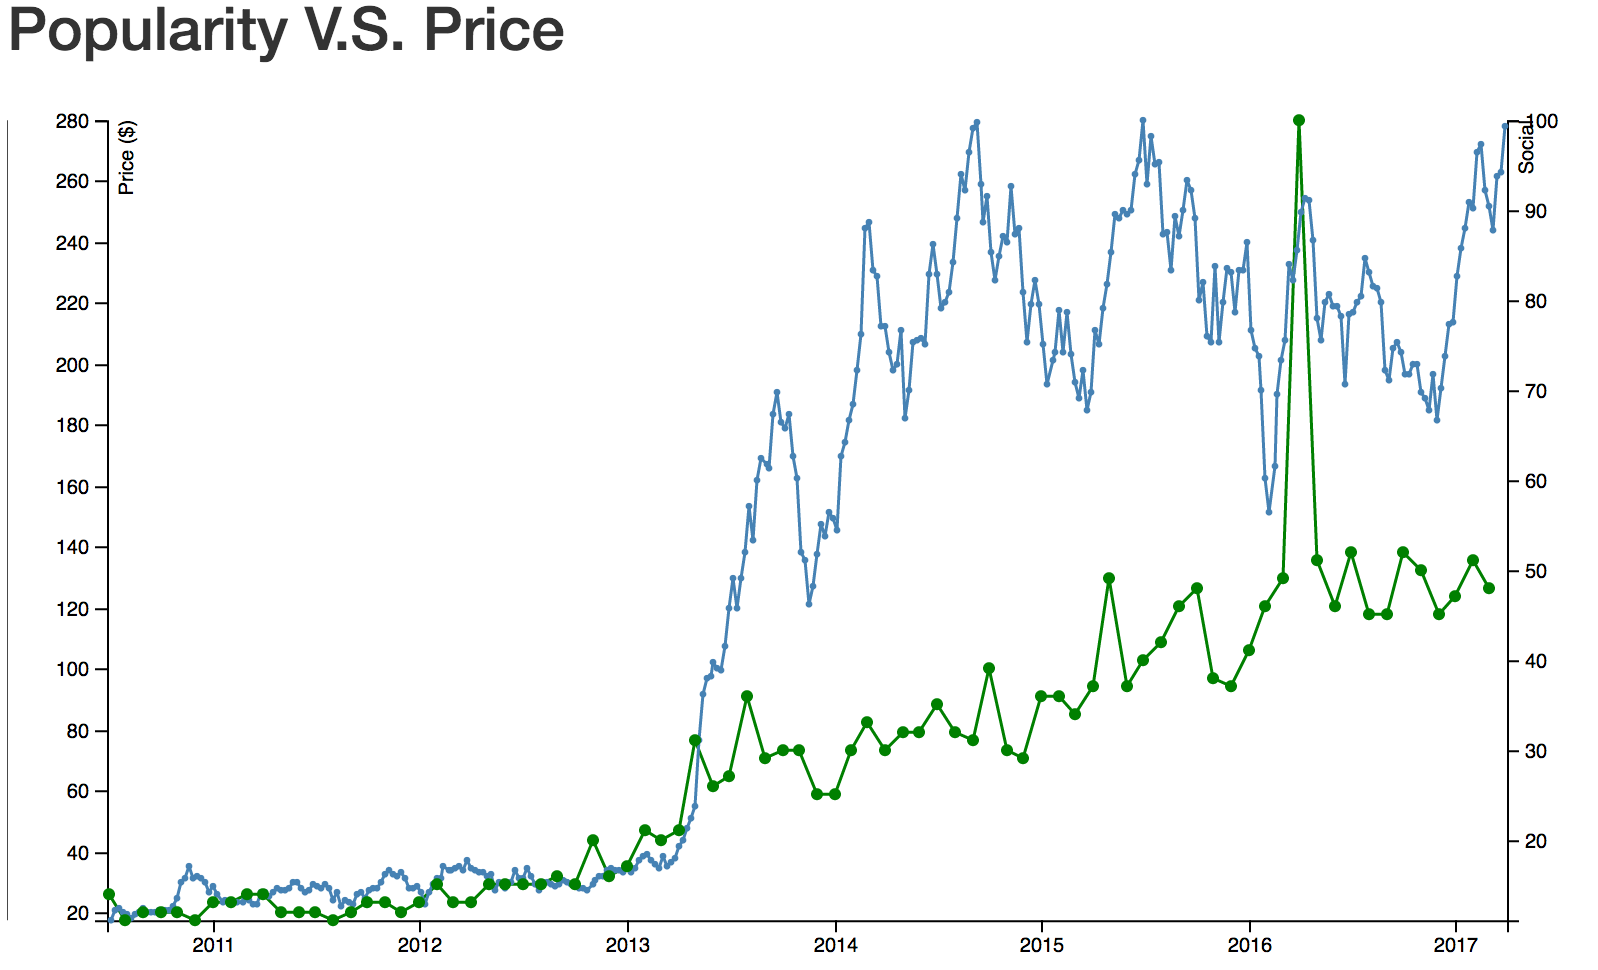
\includegraphics[height=10cm]{tesla-graph.png} 

One can display data for a specific company by using the dropdown menu
to the left of the screen. To examine the data of a specific point,
one can mouse over it. The date, and values are displayed to the right
of the screen along with a legend indicating what each line
indicates. Additionally, if one is curious about what events were
occurring at a specific point, clicking on the point will display
relevant New York Times articles from the month previous to that point
in time. 

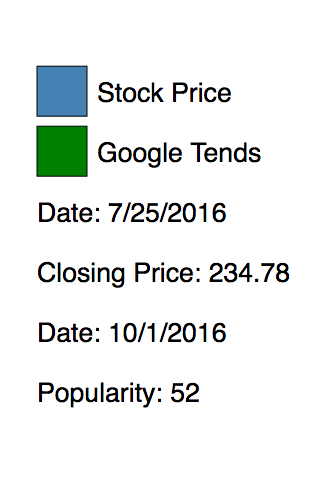
\includegraphics[height=10cm]{legend.png} 

We also included an explanation tab, which contains a description of
how to use that visualization, what it means, and how we got and
prepared our data. 

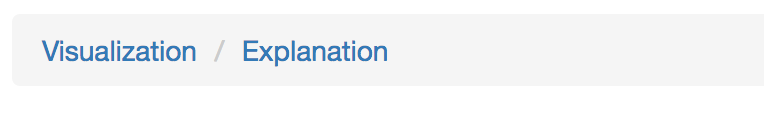
\includegraphics[height=3cm]{tabs.png} 

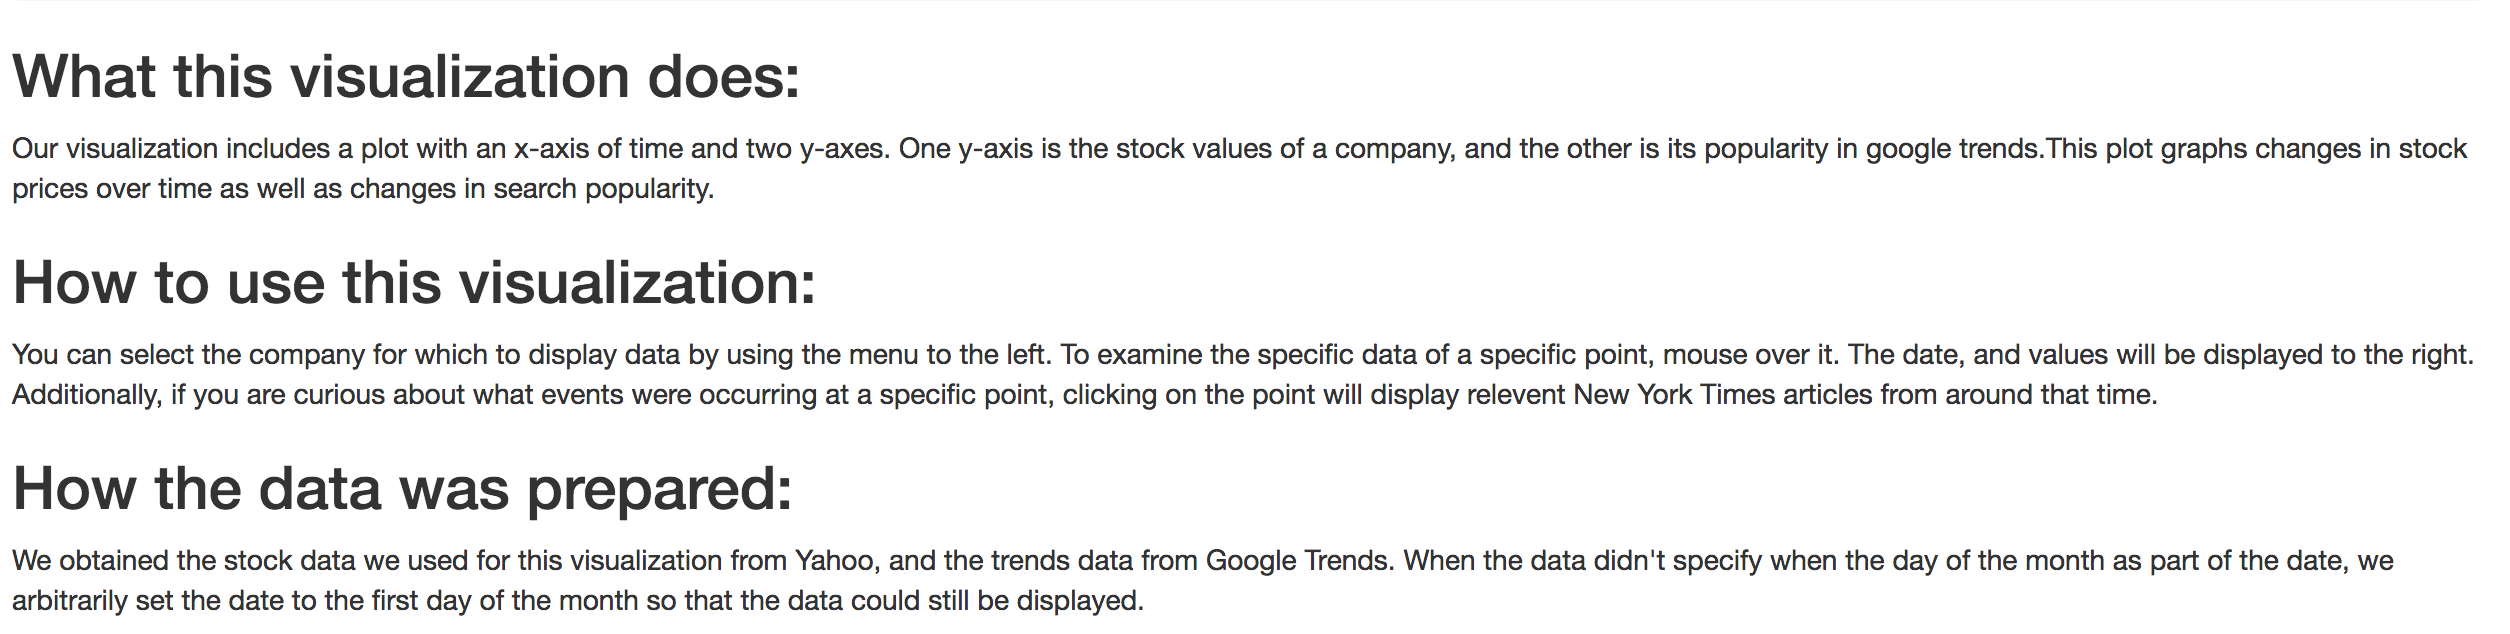
\includegraphics[height=4cm]{explain.png}

It is difficult to determine whether search interest and stock prices
are correlated overall. Although they appear to shift in similar ways
in many different scenarios, there are many times in which they appear
unrelated. We believe that we currently have too many variables
unaccounted for and too little data to make any conclusive statements
about overall correlation, although we did notice that the
relationship was more pronounced for some companies than for others. 

\item[Implementation] 

Our original design was very similar to our current design, but with
some additional features that we didn’t have the data to implement. We
originally intended to include options for the user to display
multiple lines, indicating the publicity of a company on different
social media sources, and to allow the users observe the value of all
of these sources, or filter out a select few of them, and to filter
out a select time period to look at more closely. We also originally
intended to display a map of the world, where the countries and states
were highlighted based on how many of the searches came from that
country. The final difference between our original and our final
product is that our original design did not originally include the
option of displaying new york times articles from around the time
period we are looking at. 

We originally intended for the user to be able to switch between
different interest indicators, such as Reddit, Twitter and Facebook
data, but we were unable to obtain what we were looking for from these
sources. Many of them charged a large fee for their data, if it was
publicly available at all, and we didn’t have the monetary resources
to expend on such a venture. Thus, our current product includes only
data from google trends, which cost no money and was easier to
obtain. We also realized soon that the New York Times had a free api
that would allow us to access snippets of stories in a given time
period. After becoming frustrated with the availability of Social
media data, we decided to stick to using Google trends data, and added
the ability to access New York times article from the relevant time. 

After we had found the data we wanted to use we started to work on the 
implementation, and we encountered several issues that we had to work
through. First, dates proved to be more difficult to work with than we 
intended. Creating a range of dates in javascript in order to use with
the New York Times API was not well documented, and our original 
attempt to create a date range resulted in several bugs. In addition,
we had some difficulty we didn’t expect with our stock and google 
trends data. The Amazon stocks dates were coded differently from all
the other datasets we had, using slashes instead of dashes to separate 
out the day month and year. Because of this were thus forced to
manually change the data to a format that our code could parse. This 
was done relatively quickly using Emacs macros, but discovering the
source of the error took some time. We also had several bugs that we 
eventually realized came from some google trends dates only having the
year and month and not the day. We fixed this by manually adding in 
the date “01”. Although this fixed the problem of parsing data, it
also left us with slightly unsure of the accuracy of our data. Because 
the original data didn’t include the dates, we didn’t know if our data
was shifted earlier, and if so by how much. We accounted this by 
concern by explaining what we did in the explanation part of the
visualization.  

The main way in which we used d3 in our visualization to make our 
visualization dynamic, so that users can interact with it. We feel
that this makes the user feel more connected with the data, and lets 
them choose where and how to focus their attention. We also used d3 to
add subtle transitions, which we feel make our visualization more 
aesthetically appealing. In the same vein, we used additional d3
libraries in order to provide structure and layout to the page, 
furthering its appeal. Our visualization is made almost entirely of
techniques which we learned in class, although the lines we actually 
drew in our graph, and the vertical line which appears when hovering
over the graph is not based off our work in class. We also learned how 
to work with the New York Times headlines, which are based in an
outside API.  

\item[Reflection] 

With more time, there are several potential enhancements that we could 
have made to our visualization. First, we could have added the ability
to view and compare multiple companies on the same graph. This would 
have given users another dimension of analysis with which to examine
the data, and made it easier to search for overall 
correlations. Additionally, we considered using google trends to add a
map of search locations, to help users understand how the data fits in 
spatially and whether there are any geographic trends. Lastly, we
could have made minor visual fixes and enhancements, such as adding 
more consistent animation in the New York Times data, making sure that
everything was consistent across browsers, and making adjustments so 
that the page scaled more appropriately. 
 
With more data we would have been able to improve our visualization in 
several ways. If we had been able to access the social media data
which we had originally intended to collect, we would have been able 
to include more lines in the graph and better depict publicity, as
well as show if there were discrepancies in amount of publicity across 
sites. Additionally, we would have included more data points for
google trends, so we wouldn’t have to be concerned about the error 
cause by shifting the data points to the first day of the
month. Finally, if we had access to the data, we would have added 
different metrics for evaluating the success of the companies that we
looked at. Looking at metrics like quarterly evaluations, and 
dividends would have made it easier for the user to separate out the
effects of publicity from the effects of increased profitability, as 
well as look at the connection between publicity and profitability for
different countries.  
  
  \item[Conclusion] 

Our current project provides a basic but easy to use tool for
exploring the relationship between publicity and stock prices. Because
of restrictions on data we had access too, and the amout of time we
had, we ran into limits on the sophistication of our model. However,
the current vizualization provides the data organized in a very
comprehensible way, and allows users to easily explore the connection
between publicity and stock price in the way we originally
intended. Additionally, because we include New York Times articles
from the relevent times, users can explore the context surrounding the
data in a way beyond the original socpe of our project.


\end{enumerate}
\end{document}